\documentclass[11pt]{article}
\usepackage[margin=1in]{geometry}
\usepackage[T1]{fontenc}
\usepackage{lmodern}
\usepackage{booktabs,array,tabularx}
\usepackage{amsmath}
\usepackage{graphicx}
\usepackage{xcolor}
\usepackage{listings}
\usepackage{hyperref}
\usepackage{enumitem}
\usepackage{caption}
\hypersetup{colorlinks=true,linkcolor=blue!50!black,urlcolor=blue!50!black}
\setlist{itemsep=2pt,topsep=3pt}
\captionsetup{font=small,labelfont=bf}
\definecolor{codebg}{gray}{0.96}
\lstset{language=Python,basicstyle=\ttfamily\footnotesize,backgroundcolor=\color{codebg},
  keywordstyle=\color{blue!50!black}\bfseries,commentstyle=\color{green!35!black}\itshape,
  frame=single,rulecolor=\color{gray!40},breaklines=true,columns=fullflexible,keepspaces=true,showstringspaces=false}
\newcommand{\tc}[1]{\texttt{#1}}
\newcommand{\AUCw}{\mathrm{AUC}_{\mathrm{w}}}

\title{Sub-county flood risk from NFIP data\\[2pt]\large Progress report: why NFIP, which covariates matter, simple-model results}
\author{nanoWxRisk}
\date{October 26, 2026}

\begin{document}
\maketitle

\begin{abstract}\noindent
We predict, for each Texas census block group and each heavy-rain episode (2010--2023), whether an NFIP flood claim occurs.
(1) NFIP is usable: the outcome is located at block-group level, dated to the day, has an exposure denominator, and responds to rain, insured stock and water depth in the expected direction.
(2) A plain logistic regression with six to sixteen features reaches within-event AUC $0.786$ [0.765, 0.806] on 2017--2023, against $0.5$ for any county-level model.
(3) Only two things carry that skill: the block group's own rainfall and its insured stock. Terrain, neighbourhood smoothing, location, antecedent rain and a wavelet encoder add nothing detectable.
All numbers are reproducible with \tc{scripts/51\_report\_figures.py}.
\end{abstract}

%% ------------------------------------------------------------------------------------------------
\section{Task and data}

\paragraph{Unit and label.}
We defined an \emph{episode} is a run of days (gaps $\le1$) on which a county's daily maximum gridMET rain ($4$ km) is $\ge30$ mm, with tropical-cyclone windows (HURDAT2, 800 km, $\pm2$ days) removed. A \emph{row} is a 2010-vintage block group in that county with $\ge1$ NFIP policy in force on the episode's first day. The label is $y=1$ if the block group has an inland, non-tropical NFIP claim (cause 2/3/4) dated in $[\text{start},\text{end}+2\text{ d}]$.
Result: 2,996,576 rows, 44,212 episodes, 11,264 positives (0.38\%). Train 2010--2016, test 2017--2023 (3,711 positives, 1,015 episodes), plus 7-fold CV blocked by year.
\paragraph{Problem with the tropical cyclone}
The issue with our definition is that tropical cyclones are one of the main causes of flooding in the NFIP. A tropical cyclone can bring a rain belt that sometimes spreads farther than 800 km. Human error also complicates the classification since insurance staff may not have the knowledge to distinguish between storm-caused flooding, which should include rain belt-triggered flooding, and pure inland flooding. We may need to relax our definition depending on whether we can reliably distinguish between inland or storm-triggered flooding using available data.
\paragraph{Metric.}
Within a county-episode every block group shares the county-level inputs, so we score \emph{ranking inside the episode}. With $n^1_e,n^0_e$ positives/negatives in episode $e$,
\[
\AUCw=\frac{\sum_e n^1_e n^0_e\,\mathrm{AUC}_e}{\sum_e n^1_e n^0_e},
\]
a county-level score gives exactly $0.5$. Intervals are episode-clustered bootstraps; model differences are paired.

\begin{center}\small
\begin{tabularx}{\textwidth}{@{}p{3.2cm}Xp{3.4cm}@{}}
\toprule
Source & What we take & Role \\
\midrule
NFIP claims, OpenFEMA v3 & 1.56 M national claims 2000--23; 12-digit block group, loss day, depth, damage, coverage, foundation & Outcome \\
NFIP policies, OpenFEMA v3 & Texas 11.6 M rows: effective / termination / cancellation dates, zone, coverage & Exposure per block group-day \\
gridMET & 4 km daily rain, Texas 2000--23 & Hazard \\
HURDAT2; TIGER block groups + Census 2020$\to$2010 relationship file & Tropical exclusion; one geography (2010 block groups) & Filtering, joins \\
Terrarium tiles ($\approx$150 m) & Elevation, relative height, slope at centroid & Tested covariate \\
GEFSv12 reforecast; MRMS hourly QPE & 5-member 0.25$^\circ$ rain 2010--19; 8 hourly events & Forecast-mode and interpolation tests \\
\bottomrule
\end{tabularx}
\captionof{table}{Datasets in the flood pilot (SCS-line data, ERA5 and IFS ENS, are not covered here).}
\end{center}

%% ------------------------------------------------------------------------------------------------
\section{Why NFIP is a reasonable outcome}

\paragraph{Spatial and temporal resolution.}
Claims carry a 12-digit \tc{censusGeoid} (96--99.7\% populated) and an exact loss date. Latitude/longitude are rounded to one decimal ($\approx$11 km) and are not used; the \tc{geoid} is the only location key. Figure~\ref{fig:tx} maps the claims inside our episode windows onto 2010 block-group polygons: 5,307 of the 14,290 block groups in the table have at least one such claim, concentrated on the Gulf coast, Houston, San Antonio--Austin and Dallas--Fort Worth, which matches where flooding and insured stock are. Notice that Spatial resultion is not even, this may induce bias on location.

\begin{center}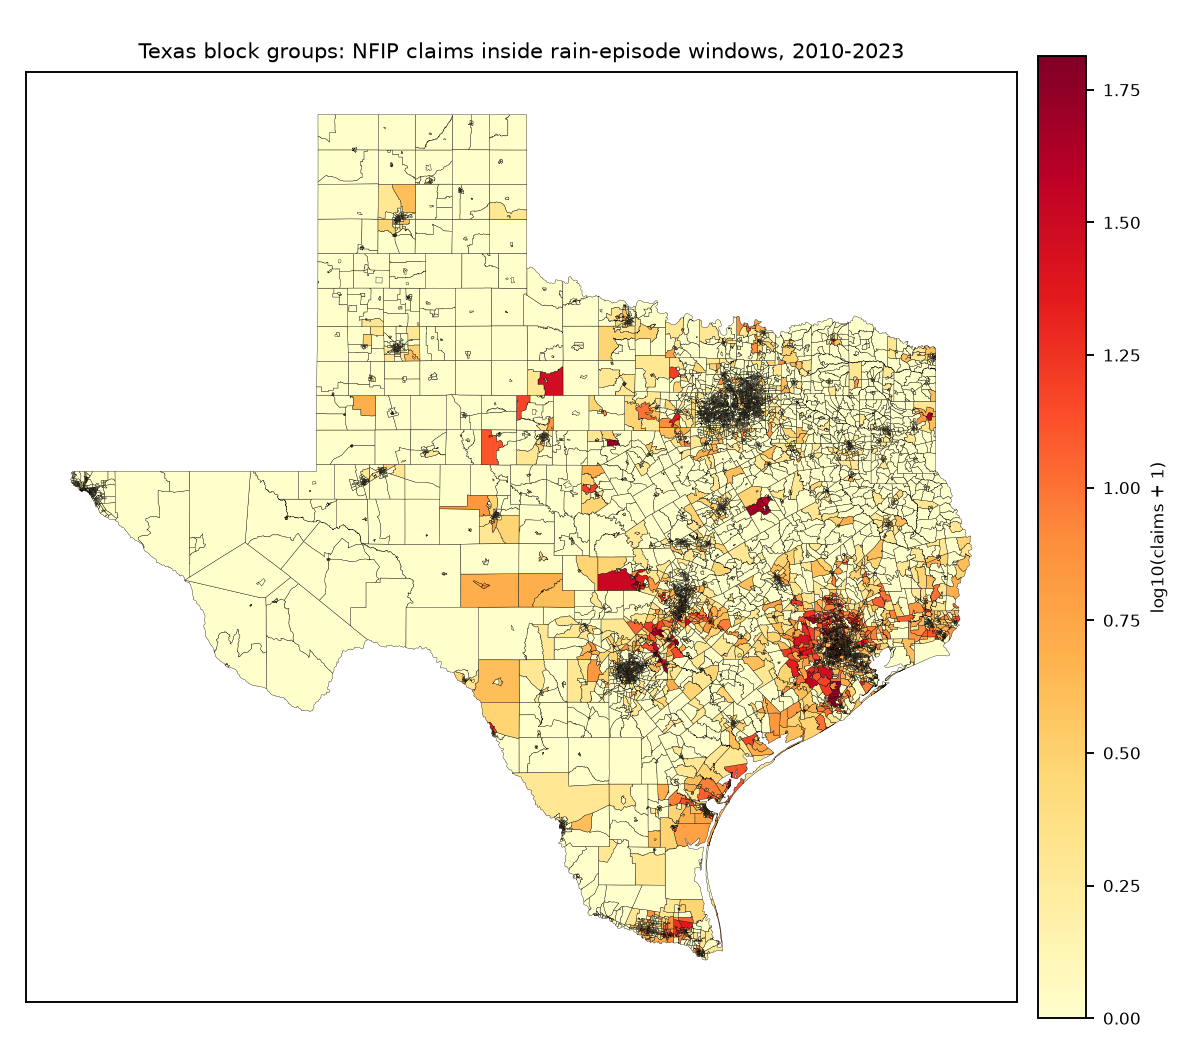
\includegraphics[width=0.62\textwidth]{figs/fig_texas_claims.png}
\captionof{figure}{Texas block groups coloured by NFIP claims inside episode windows, 2010--2023 (polygons: 2010 TIGER; key: 12-digit GEOID).}\label{fig:tx}
\end{center}

\paragraph{Does the outcome respond to hazard and exposure?}
Figure~\ref{fig:dose} shows three monotone relations computed from the data: the share of block groups with a claim rises from 0.04\% (cell rain $\le30$ mm) to 17.8\% ($>150$ mm); it rises with the number of policies in force (0.05\% for one policy to 0.80\% for $>300$); and for single-family homes the median damage-to-coverage ratio rises from 0.15 (interior depth $\le6$ in) to 0.56 ($>48$ in), Spearman $0.34$ ($n\approx150{,}000$). Raw dollar amounts, by contrast, are nearly uncorrelated with intensity (county-level dollars vs.\ rain: 0.03), so we model occurrence and normalise losses by coverage.

\begin{center}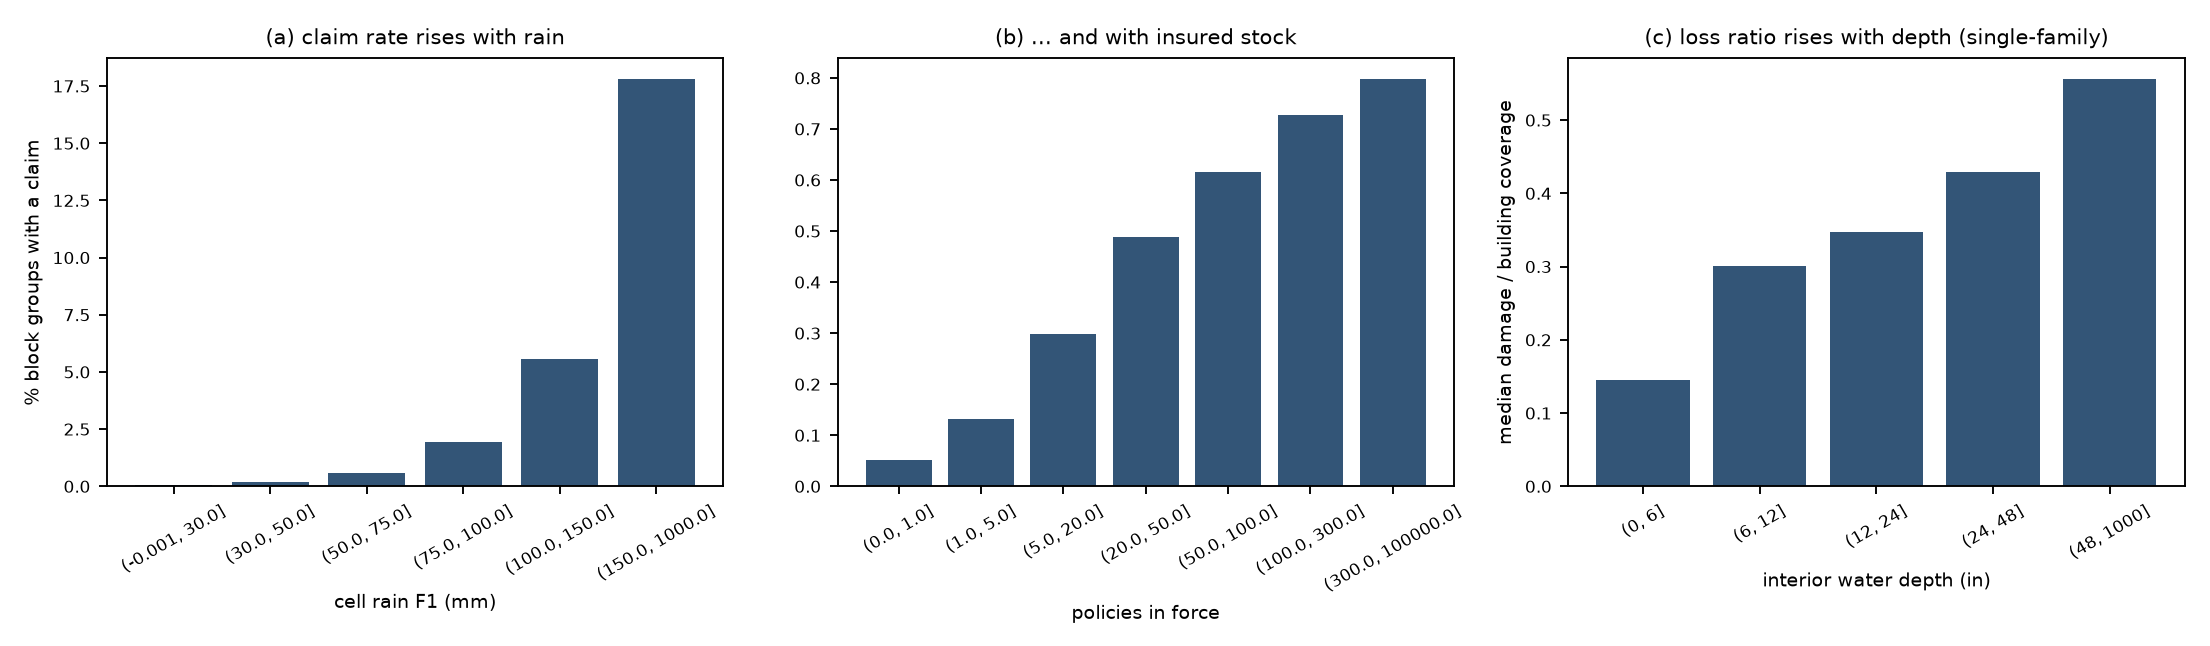
\includegraphics[width=\textwidth]{figs/fig_dose_response.png}
\captionof{figure}{(a), (b): block-group claim rate by cell rain and by policy count (training+test table). (c): all NFIP single-family claims with interior depth reported, median of building damage / coverage.}\label{fig:dose}
\end{center}

\paragraph{Internal consistency checks.}
\begin{itemize}
  \item Labels shuffled within episodes: $\AUCw$ falls from $0.781$ to $0.501$ (no pipeline leak).
  \item No claim occurs in a block group without a policy in force that day (0\%); episode windows contain 88.8\% of Texas claims 2010--2023.
  \item $\AUCw$ is stable at 0.78--0.80 under the trigger threshold (30 vs.\ 50 mm), tropical window (800 vs.\ 1200 km), and claim-to-polygon mapping confidence.
  \item The worst of seven year-blocked CV folds is $0.751$.
\end{itemize}

\paragraph{Known weaknesses}
\begin{itemize}
  \item \emph{Mixed geography}: NFIP block-group codes mix 2010 and 2020 vintages (Texas claims match 90.2\% to 2010 alone, 70.1\% to 2020 alone). We map with the Census overlap file by largest land share: 100\% matched, 92--99\% with share $\ge0.8$.
  \item \emph{Exposure}: the policy file starts with 2009 effective dates, so denominators start in 2010; 409,641 of 410,241 cancelled policies end early, so ``in force'' uses the earlier of expiry and cancellation (counts were 2.6\% too high).
  \item \emph{Placeholders}: depth 0 (large damage recorded at 0), 999/99 codes and \tc{foundationType}$=0$ are nulled and flagged, not read as ``dry'' or ``no foundation''. Exterior depth is missing for 96--100\% of claims before 2016.
  \item \emph{Label drift}: claims per million policy-episodes are 621 (2015) and 710 (2016) against 15--24 in 2011, 2020, 2022; the positive rate is 0.58\% in training and 0.22\% in test. We therefore report ranking metrics, not cross-year probabilities.
  \item \emph{Selection}: rows are insured block groups only, i.e.\ the conditional sample ``insured exposure''.
\end{itemize}


%% ------------------------------------------------------------------------------------------------
\section{How inland flood is isolated}

NFIP does not label ``inland flood'' directly, so we use two independent kinds of evidence and check one against the other (\tc{scripts/52\_inland\_filter\_audit.py}; Texas claims 2010--2023 mapped to 2010 block groups, $n=151{,}216$).

\paragraph{Evidence 1: what the dataset marks.}
\begin{itemize}
  \item \emph{Cause of damage}: we keep codes 2 (river/lake overflow), 3 (alluvial fan) and 4 (rainfall ponding), and drop 1 (tidal overflow, 4,131 claims), 0 (other, 38,967) and the landslide/erosion codes. This leaves 105,289 claims.
  \item \emph{Event name} (\tc{floodEvent}): drop claims whose name matches a tropical-cyclone pattern (``hurricane'', ``tropical'', named storms; word-bounded so that ``ian'' does not match Florida or Louisiana). 70,300 of the 105,289 inland-cause claims (66.8\%) are named: Hurricane Harvey 61,311, Imelda 7,531, Hanna 773, Beta 242, Bill 196.
\end{itemize}
The cause code alone is therefore not enough: Harvey's rainfall ponding and river flooding are coded 2/4, exactly like a non-tropical flash flood. The name field fixes this, but it is blank for 16,498 inland claims (15.7\%).

\paragraph{Evidence 2: our storm-track filter.}
For each county and day we flag \emph{tropical-cyclone influence} if any HURDAT2 best-track point (Atlantic and eastern Pacific) lies within 800 km of the county centroid within $\pm2$ days. This is independent of NFIP: it uses only track data and geography. It is applied to the rain side, so a county-day inside the window cannot start an episode (6,441 of 99,445 county-days with daily rain $\ge30$ mm, 6.5\%, are removed), and all claims in such a window are excluded.

\paragraph{Cross-check.}
\begin{center}\small
\begin{tabular}{@{}lrr@{}}
\toprule
Inland-cause claims (105,289) & Track-flagged & Not flagged \\
\midrule
Named tropical & 70,008 & 292 \\
Not named (blank or non-tropical name) & 1,625 & 33,364 \\
\bottomrule
\end{tabular}
\captionof{table}{Name filter vs.\ track filter. 99.6\% of named claims are inside the track window; 1,622 of the 1,625 flagged-but-unnamed claims have no event name at all.}
\end{center}
The two filters agree on 70,008 + 33,364 = 103,372 claims (98.2\%). Disagreements are small and have a clear reading: the 1,625 unnamed claims inside a track window are the cases where the name field is missing for a tropical event, and the track filter removes them; the 292 named claims outside the window are removed by the name. Of the 16,498 claims without an event name, 14,876 (90\%) lie outside every track window, which is independent support that most unnamed claims are not tropical. Name alone keeps 34,989 claims; adding the track filter leaves 33,364. The label used in the pilot is the name-based set (the stored table, 31,057 of the 34,989 claims inside episode windows), with the track filter acting at the episode level.

The same check from the other side: tidal-overflow claims (cause 1), which should be tropical-driven, are 88\% inside the track window, so the track filter does capture surge-type events and is not tuned to the NFIP labels.

\paragraph{Sensitivity and limits.}
A wider filter (1200 km, $\pm4$ days) leaves $\AUCw$ unchanged (L2 0.785 vs.\ 0.786), so the result does not depend on the exact radius. The residual risk is a tropical remnant that is both unnamed and outside the window (not quantifiable here, and a small share given the numbers above), and a non-tropical flood that happens to fall inside a 800 km / 2-day window, which we remove at some cost in sample size.

\begin{lstlisting}
TC_PATTERN = r"(?i)\b(hurricane|tropical|typhoon|post-tropical|harvey|imelda|...)\b"
inland = claims.cause.isin(["2", "3", "4"]) & ~claims.flood_event.fillna("").str.contains(TC_PATTERN)   # evidence 1

d = great_circle_km(county_centroid, track_point)                  # evidence 2, per HURDAT2 point
tc_flag[day-2 : day+3, counties[d <= 800]] = True                  # tropical influence for +-2 days
trig = (county_daily_max_rain >= 30) & ~tc_flag                    # episodes cannot start in a flagged window
\end{lstlisting}

Additionally, due to the differences in geography between the states, this means that, under the current assumption, we must limit ourselves to states that share some geographic features. For example, the East Coast and the Southwest desert states.

%% ------------------------------------------------------------------------------------------------
\section{Covariates: what works and what does not}

\paragraph{Candidate features.}
Rain at the block group's grid cell (largest day $F1$, largest 3-day $F3$, total $S$, 14-day antecedent), neighbourhood statistics around the cell ($3/7/15$-cell means and maxima, exceedance fractions), county-level rain, exposure (log policies in force, SFHA share, single-family share, mean coverage), location and log area, centroid terrain, and wavelet scale features. Linear models use a fixed transform plan (\tc{log1p} for rain and counts, \tc{asinh} for signed heavy tails, month as $\sin/\cos$) fitted on 2010--2016 only; trees use raw features.

\paragraph{Simple models.}
Table~\ref{tab:min} shows how far very small models go; Figure~\ref{fig:cov} shows single-feature scores, the coefficients of the 16-feature logistic model, and what each feature group adds.

\begin{center}\small
\begin{tabular}{@{}lc@{}}
\toprule
Model (logistic regression, test 2017--2023) & $\AUCw$ [95\% CI] \\
\midrule
County rain only & 0.500 \\
Policy count only & 0.662 [0.643, 0.683] \\
Cell rain only ($F1$) & 0.740 [0.712, 0.765] \\
Policy count + cell rain & 0.778 [0.756, 0.799] \\
Exposure (4 features) + cell rain (4 features) & 0.784 [0.761, 0.804] \\
+ county rain, calendar (16 features) & 0.786 [0.765, 0.806] \\
Boosting, depth 5, same features & 0.786 \\
\bottomrule
\end{tabular}
\captionof{table}{Two features give $0.778$; sixteen give $0.786$; a boosted tree gives the same. The model is limited by information, not capacity (learning curve at 2/4/7 training years: 0.774/0.768/0.781).}\label{tab:min}
\end{center}

\begin{center}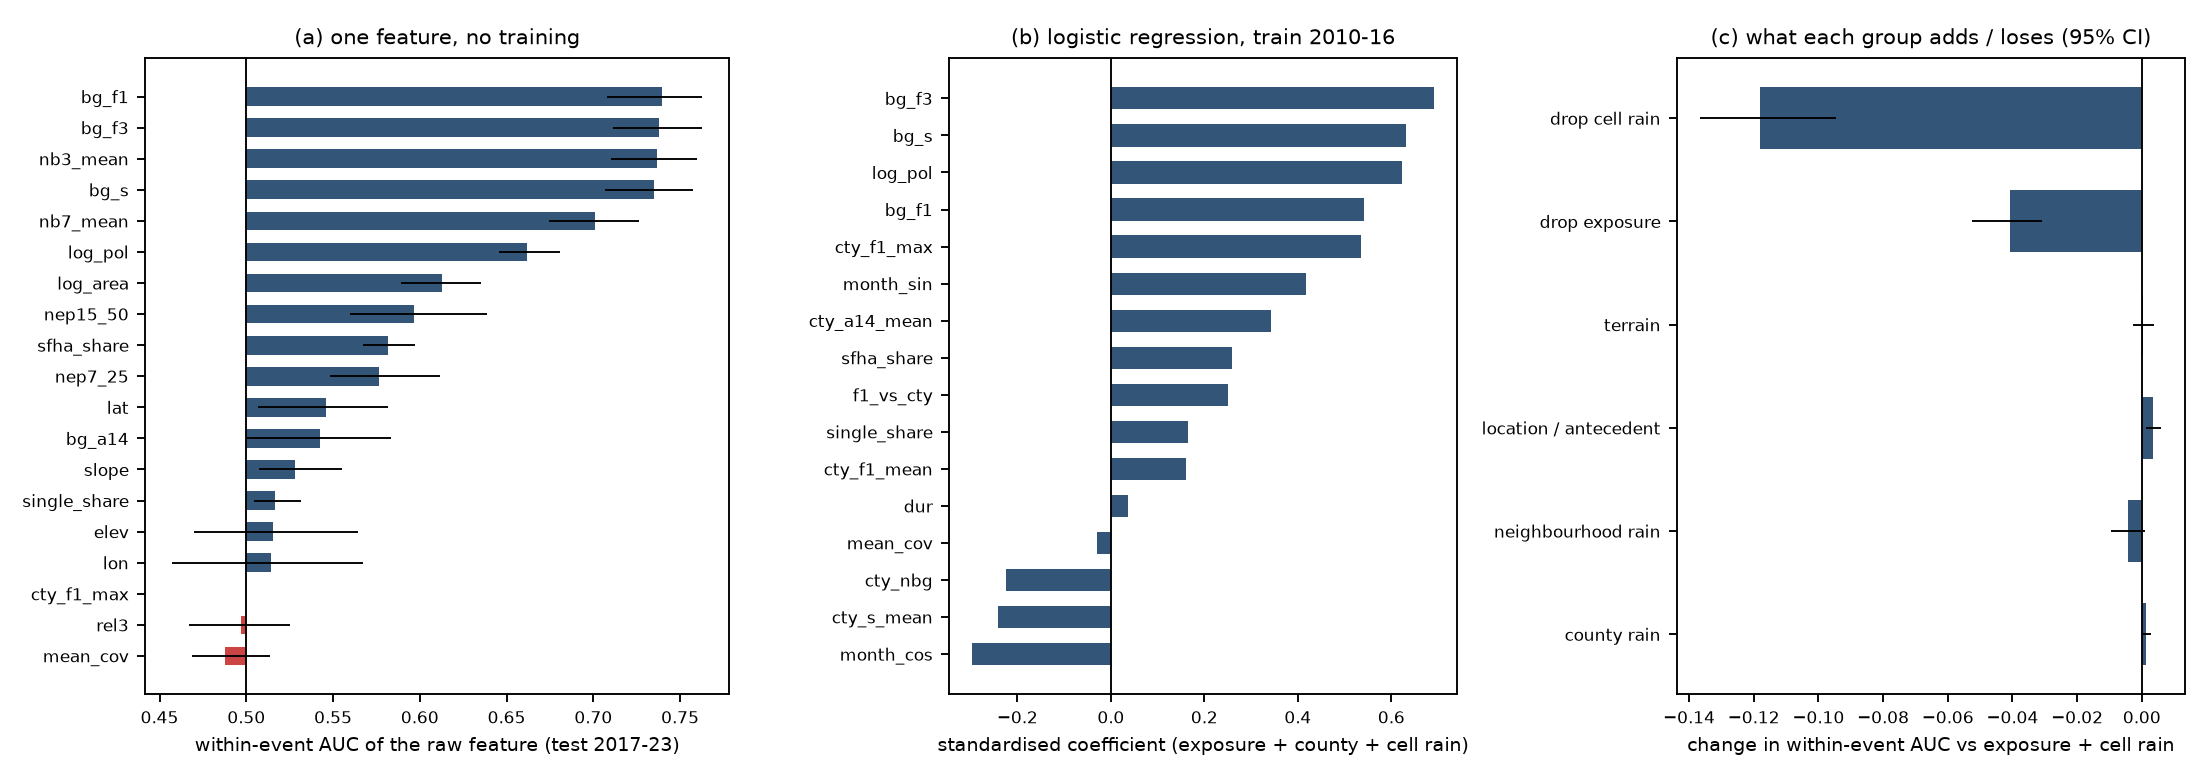
\includegraphics[width=\textwidth]{figs/fig_covariates.png}
\captionof{figure}{(a) Within-event AUC of each raw feature, no training (county-constant features give 0.5 by construction). (b) Standardised logistic coefficients. (c) Change in $\AUCw$ relative to exposure + cell rain: groups added, or exposure / cell rain removed. Event-clustered 95\% bootstrap.}\label{fig:cov}
\end{center}

\paragraph{Useful.}
\begin{itemize}
  \item \textbf{Cell rain} (+0.118 [0.095, 0.137] when removed from the model): $F1$, $F3$ and $S$ are essentially one signal (single-feature AUC 0.735--0.740; variance inflation up to 184), which is why their coefficients in (b) are individually large and should not be read separately.
  \item \textbf{Exposure} (+0.041 [0.031, 0.052] when removed), mostly log policy count (0.662 alone); SFHA share is weaker (0.582); log area carries 0.613 mostly as a proxy for stock.
  \item \textbf{Flood history}: claims in the block group 2000--2009 and in the prior 3 years add $+0.026$ [0.020, 0.033] with observed rain and $+0.051$ [0.023, 0.075] with forecast rain. Not yet in the main model; partly a proxy for flood zone and take-up.
\end{itemize}

\paragraph{No detectable value.}
\begin{itemize}
  \item \textbf{Neighbourhood rain} ($-0.004$ [$-0.010$, $+0.001$]): for \emph{observed} rain, the point value already contains the information.
  \item \textbf{Centroid terrain} (+0.0003 [$-0.003$, $+0.004$]; also null in forecast mode, and not explained by the flood-zone share).
  \item \textbf{County rain, season}: constant inside an episode, so linear coefficients cannot change within-event ranking (+0.001 [0.000, 0.003]).
  \item \textbf{Location and antecedent rain}: $+0.004$ [0.001, 0.006], statistically positive but negligible; history absorbs it.
  \item \textbf{Wavelet scale features, exposure composition (new vs.\ mid-age policies), economic covariates (rates, prices, permits, sales), group-aware scaling}: intervals span zero in earlier stages (wavelet $+0.003$ [$-0.000$, $+0.006$]).
  \item \textbf{Mean coverage}: single-feature AUC $0.488$ and coefficient $\approx0$.
\end{itemize}

\paragraph{Spatial picture.}
Figure~\ref{fig:map} places the simple model on block-group polygons for one county-episode in the test period (Cameron County, 24 June 2019; 220 block groups, 48 with a claim). It is the largest-rain-variation episode among test episodes with $\ge150$ block groups and $\ge25$ positives, chosen by that rule before looking at scores, so it is an illustration, not a typical case: here $\AUCw=0.98$. The model recovers the rain gradient from the north-west; the inland block groups with high rain and enough policies are the ones marked.

\begin{center}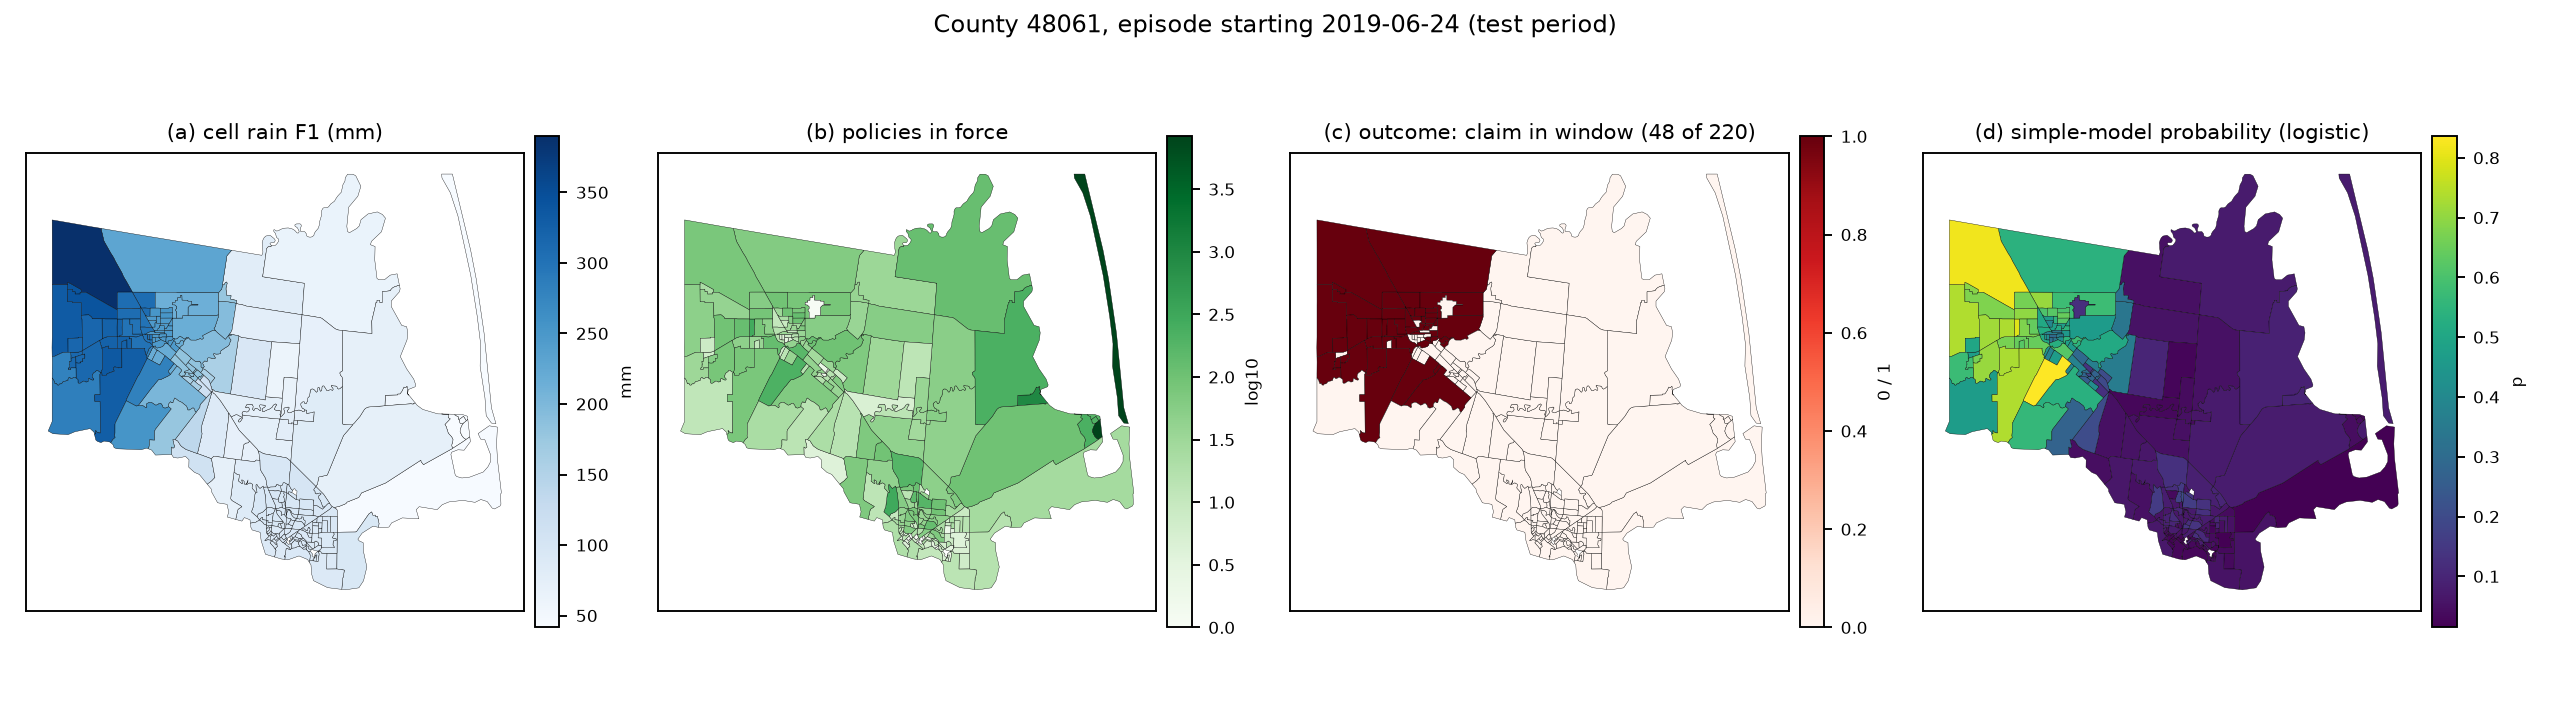
\includegraphics[width=\textwidth]{figs/fig_county_episode.png}
\captionof{figure}{One test episode on block-group polygons: (a) cell rain, (b) policies in force, (c) outcome, (d) logistic-regression probability.}\label{fig:map}
\end{center}

\paragraph{Forecast mode.}
Replacing observed rain by a GEFSv12 5-member forecast (leads 36--84 h, 0.25$^\circ$, 2017--2019 test, 497 episodes) gives: exposure only 0.622, observed 4 km 0.736, observed averaged to 0.25$^\circ$ 0.712, forecast mean 0.667. About 40\% of the rain gain survives; about 0.024 is lost to resolution and 0.045 to forecast error. Member votes, spread and neighbourhood probabilities add $+0.002$ [$-0.017$, $+0.016$].

%% ------------------------------------------------------------------------------------------------
\section{Data snippet}

Rows of the pilot table for one test episode (Cameron County, 24 June 2019; selection as above), sorted by rain. \tc{bg10}: 12-digit block-group GEOID (2010); \tc{bg\_f1}: cell rain (mm); \tc{nb7\_mean}: $7\times7$ mean; \tc{n\_pol}: policies in force.

\begin{lstlisting}[basicstyle=\ttfamily\scriptsize,language={}]
bg10          y n_claims  bg_f1  nb7_mean  cty_f1_max  n_pol  sfha_share  mean_cov  area_km2
480610103012  1       15  389.7     317.7       416.4     78       0.359     0.175   104.397
480610103011  1        9  340.8     310.3       416.4     22       0.455     0.140     2.010
480610103021  1       14  340.8     310.3       416.4     40       0.000     0.184    19.029
480610118022  0        0  218.9     211.8       416.4     14       0.000     0.094     1.541
480610130042  0        0   96.1      71.4       416.4      7       0.000     0.175     0.243
480610123043  0        0   41.6      43.0       416.4    201       0.687     0.290     0.702
480610123041  0        0   41.6      43.0       416.4    170       0.576     0.471     0.673
\end{lstlisting}

NFIP claim and policy rows (Texas, public, redacted):

\begin{lstlisting}[basicstyle=\ttfamily\scriptsize,language={}]
CLAIM   dateOfLoss  censusGeoid   cause extDepth bldgDamage bldgCoverage occ foundation elevated
        2017-08-27  482013430001  4     11.0     68000      53000        11  1          False
        2017-08-28  482014221005  4      0.0     19657      250000       11  1          False   <- depth 0 is not "dry"
POLICY  censusGeoid   effective   termination cancelled zone occ coverage foundation postFIRM
        482014227012  2018-04-13  2019-04-13  None      AE   1   99700    1          False
        480717102002  2020-06-30  2021-06-30  None      X    1   250000   1          True
\end{lstlisting}

%% ------------------------------------------------------------------------------------------------
\section{Code snippet}

Episode detection and block-group sampling (\tc{scripts/25}); full scripts are in the repository.

\begin{lstlisting}
trig = (D1 >= T) & ~tc                         # county daily max >= 30 mm, outside tropical window
cut  = np.flatnonzero(np.diff(idx) > 2)        # a gap of more than one dry day starts a new episode

bgs = bgs[n_pol[bgs, es] >= 1]                 # rows: block groups with >= 1 policy in force
F1  = sl[2:].max(axis=0)                       # largest daily rain, full 4 km field
yy, xx = iy[bgs], ix[bgs]                      # grid cell of each block-group centroid
y   = ((C[bgs, w1 + 1] - C[bgs, w0]) > 0)      # claim in [start, end + 2 d] from cumulative claim array
row = {"bg_f1": F1[yy, xx], "nb7_mean": uniform_filter(F1, 7)[yy, xx],
       "n_pol": n_pol[bgs, es], "sfha_share": n_sfha[bgs, es] / n_pol[bgs, es], "y": y}
\end{lstlisting}

Policies in force as a difference array, and the metric (\tc{wxrisk.flood\_pilot}, \tc{scripts/26}):

\begin{lstlisting}
up = np.bincount(bi*(n+1) + s0, weights=w, minlength=nb*(n+1))     # +w on effective day
dn = np.bincount(bi*(n+1) + s1, weights=w, minlength=nb*(n+1))     # -w on coverage_end (min of expiry, cancellation)
in_force = np.cumsum((up - dn).reshape(nb, n+1), axis=1)[:, :n]    # [block group, day]

def within_auc(ep, y, s, min_bg=10):          # pooled, pair-weighted
    for _, g in pd.DataFrame({"ep": ep, "y": y, "s": s}).groupby("ep"):
        n1 = g.y.sum(); n0 = len(g) - n1
        if len(g) < min_bg or n1 == 0 or n0 == 0: continue
        r = rankdata(g.s); auc = (r[g.y == 1].sum() - n1*(n1+1)/2) / (n1*n0)
        num += auc*n1*n0; den += n1*n0
    return num / den

tr, te = year <= 2016, year >= 2017            # split by year
lr = LogisticRegression(C=0.1).fit(Z[tr], y[tr])   # Z = PILOT_PLAN transform fitted on train rows only
\end{lstlisting}

%% ------------------------------------------------------------------------------------------------
\section{Caveats and next steps}

\begin{itemize}
  \item One state, one split; 2015--2016 dominate training; test intervals about $\pm0.02$--$0.03$. Selected-county figure is illustrative only.
  \item Rain is the gridMET \emph{daily} value at the centroid: no sub-daily intensity, no area average; terrain is centroid-only. Drainage and building footprints are not in the data.
  \item Occurrence only; no payout or cross-year absolute probability. Forecast mode uses a fixed reforecast with five members.
  \item Next: add flood history and block-group building priors (elevated share, known-foundation shares plus an explicit unknown share) to the main model; FEMA NFHL zone and HAND at building footprints in place of centroid terrain; finer or longer-lead forecasts; a second state (LA, FL, SC); a separate level model (episode claim count $\times$ within-event share).
\end{itemize}

\end{document}
